\section{実験}
\label{sec:exp}
提案手法をマルウェアに適用して実験を行った.本章では,この実験の目的,方法,結果について解説する.また,結果に対する考察も述べる.
\subsection{実験の目的}
本研究の提案手法により得たマルウェアの実行ログから,マルウェアの挙動を明らかにできていることを示す.

\subsection{実験方法}
今回,11 個の検体を用いた実験と,SMS を送るマルウェア (1 つのマルウェア)を用いた実験の 2 種類の実験を行った.それぞれの実験方法の説明の前に\ref{expmalware} で,実験に用いたマルウェアがどのような挙動を示すかを示す.それぞれの実験については,\ref{exp1} , \ref{exp2} で詳しく説明する.

\subsubsection{実験に用いたマルウェア}
\label{expmalware}
今回の実験に用いたマルウェアの挙動を以下に示す \cite{golddream} \cite{basebridge} \cite{droiddreamlight} \cite{crazyapp} \cite{icalendar} \cite{snake} \cite{trojan} . これらのマルウェアはインターネット上のサイト \cite{malwaresite} からダウンロードした.

\begin{enumerate}
\item GoldDream
	\begin{itemize}
	\item	receiver を使うことで,SMS,電話等のシステムイベントをバックグラウンドで監視し,送信元のアドレス,電話,SMS のタイムスタンプ,電話番号をファイルに保存した後,外部のサーバへそのファイルを送信する.
	\item 外部のサーバから 4 種類のコマンドを受け取り,それを実行する.
	\begin{enumerate}
		\item SMS をバックグラウンドで送信する
		\item 電話を発信する
		\item アプリをインストールまたはアンインストールする
		\item ファイルを外部のサーバへアップロードする
	\end{enumerate}
	\end{itemize}

\item basebridge
	\begin{itemize}
	\item アプリのアップグレードを促すダイアログを出し.そこでアップグレードを選択すると,basebridge は com.android.battery を感染した端末にインストールする.
	\item 外部のサーバとの通信を行い,番号などが載った configuration list  をダウンロードし,この情報を基に,SMS を送信する.
	\item SMS をバックグラウンドで送信したことをユーザに気付かれないようにするために,モバイルキャリアからの課金確認の SMS をブロックする.
	\end{itemize}

\item com.tencent.qqgame
	\begin{itemize}
	\item 挙動は GoldDream と同じ
	\end{itemize}

\item Beauty Breast
	\begin{itemize}
	\item 感染した端末に電話がかかってくると,その端末の端末番号,機種名,SDK バージョン等の端末の情報を外部サーバへ送る.
	\item 新しいパッケージのインストールと,それを促すプロンプトを表示する.
	\item マルウェア自身では,上の挙動をすることはなく,ユーザの何らかの操作無しでは実行されない.
	\end{itemize}

\item Beauty Leg
	\begin{itemize}
	\item Beauty Breast と挙動は同じ.
	\end{itemize}

\item Beauty Girl
	\begin{itemize}
	\item Beauty Breast と挙動は同じ.
	\end{itemize}

\item crazy app
	\begin{itemize}
	\item 感染した端末の IMEI (端末を識別する番号) を外部サーバへ送信する.
	\item  ブラウザのブックマーク情報とブラウザの閲覧履歴をアップロードする.
	\end{itemize}
\item iCalendar
	\begin{itemize}
	\item 有料サービスに登録させるためにある番号へ SMS をバックグラウンドで送信する.
	\item SMS  を送信できたかどうかをタグとして内部で記録している.
	\item ユーザに気づかれるのを防ぐために一度しか行われない.
	\end{itemize}
	
\item iMatch
	\begin{itemize}
	\item 挙動は iCalendar と同じ.
	\end{itemize}
	
\item Snake App
	\begin{itemize}
	\item バックグラウンドで外部サーバに端末の GPS 情報を送信する.
	\item 表向きはゲームアプリとして振舞っている.
	\end{itemize}
	

\item com.tencent.qq
	\begin{itemize}
	\item 感染した端末の IMEI 番号,電話番号,登録者 ID,SIM カードのシリアル番号を盗み,外部のサーバへ送信する.
	\item 過去に SMS を送った電話番号を収集する.
	\item 外部のサーバからコマンドを受け取り,以下の動作を行う
	\begin{enumerate}
		\item SMS コンテンツや URL をサーバから受け取った電話番号へ送信する.
		\item ある URL から APK ファイルをダウンロードし,それをインストールする.
		\item ブラウザにブックマークを追加する.
		\item ある URL へ誘導するポップアップを表示する.
	\end{enumerate}
	\item ログファイルに記載されている電話番号からの SMS をブロックする.
	\end{itemize}
\end{enumerate}

\subsubsection{実験 1:11 個の検体を用いた実験}
\label{exp1}
実験 1 では\ref{expmalware} で挙げた 11 個の検体に対して,\ref{methodtop} で述べた手法を適用し.それぞれのマルウェアを実機で実行してログから挙動を解析できるかどうかを実験する.

実際にマルウェアにログコードを挿入する前の準備として,ログコードを挿入するクラスを絞り込む.なぜこの処理が必要であるかというと,マルウェアのソースコード中の全てのクラスのメソッドにログコードを挿入してしまうと,不必要なログが大量にでてきてしまうためだ.例えば,ゲームアプリの場合,常に描画のためのメソッドが実行されている.このようなメソッドと不正を動きをしているメソッドのログが混ざって出力されてしまうと,解析が非常に行いづらい.マルウェアのソースコード ( Java クラスファイル) を探索し,"install", "download", "SMS", "remote" などのマルウェアの代表的な挙動を表す単語を含むメソッドのクラスを不正な動きをするクラスとみなし,コードを挿入するクラスとする.

コードを挿入するクラスを決定したら,そのクラスのメソッドの先頭にログコードを挿入した.ログコードが挿入されたマルウェアを Nexus 5 (Android 4.4.4) にインストールした後,手動でそれぞれのマルウェアを起動した.

\subsubsection{実験 2:SMS  を送るマルウェアの実験}
\label{exp2}
実験 2 では,\ref{methodtop}, \ref{methodcalls} の 2 つの手法を適用する.この実験では SMS を送るマルウェアである iMatch に対してのみ行った.実験 1 と同様にコードを挿入するクラスを決定した後に,そのクラスのメソッドに対して,メソッド呼び出しの前後にログコードを挿入した.その後,メソッドの先頭へログコードを挿入する.これも実験 1 と同じ操作である.そして,ログコードを挿入した iMatch を Nexus 5 (Android 4.4.4) にインストールして,これを起動した.

\subsection{実験結果}
\subsubsection{実験 1 の結果}
11 個中,8 個のマルウェアからログを得ることができた.その 8 個の中の 5 個では,不正な動きを示すログを得ることができた.これら 5 つの結果を以下に示すと同時に,得られた結果と\ref{expmalware} との比較を述べる.その他についても,原因について考察する.
\begin{enumerate}
\item GoldDream \mbox{}\\
	3 種類のメソッドのログを得ることができた.図\ref{zjservicereceive}, 図\ref{zjserviceuseragent}, 図\ref{zjservicegetkey} は,この実験で GoldDream から得られたログである.メソッドの説明.いつどのように実行されるか.
	
	\ref{expmalware} との比較
	
\item com.tencent.qqgame \mbox{}\\
	2 種類のメソッド,getCommunicator, isConnected のログを得ることができた.この結果を図\ref{qqgame} に示す.この 2 つのメソッドはこのアプリの画面からホーム画面へ戻る操作をしたときに,この 2 つのメソッドが同時に実行される.getCommunnicator メソッドにより, 何らかの通信コネクションを表すオブジェクトを取得していることがわかる.また,図\ref{qqgame} の 3,4 行目から,isConnected メソッドは SocketCommunicator クラスのメソッドであることが読み取れる.よって,このマルウェアが外部の通信を試みようとしていて,このメソッドで通信が確立されているかを確かめていることがわかる.
	
	今回の実験では \ref{expmalware} で述べた挙動の一部をログによって明らかにすることができた.この結果には 2 つの原因があると考えられる.まず 1 つは,マルウェアが実行したときには,外部サーバが動いていなかったことである.マルウェア作成者が何らかの理由ですでに外部サーバを停止させた可能性がある.もう一つは.この実験で用いた Nexus 5 には SIM カードが入っていないためである.そのため,今回の実験環境は,このマルウェアが監視している電話の着信,SMS の受信などのイベントが発生しない環境であった.つまり,マルウェアが電話や SMS の情報を収集しようとしてもその情報がない.
\item iCalendar \mbox{}\\
	得られたログの結果を図\ref{calendar} に示す.SMS を送信していることを示すメソッド sendSms のログを得ることができた.このメソッドはアプリが起動した状態で画面を 5 回タップすると実行される.このメソッドが実行された時は画面には何も表示されない.何度かインストールを行うことで,このメソッドがインストール後一回のみ実行されることも確認した.
	
	しかし,SMS が送られたかどうかを記録する挙動のログは今回の実験では得ることができなかった.Android 端末だけでなくモバイル端末は SIM カードがないとSMS を送信することができない.実験で使用した Nexus 5 には SIM カードが挿入されていなかったために SMS が送信できなかった.そのため,送信ができなかったという記録をする挙動をしてもよいはずである.この動作をするクラスにログを挿入していなかったため,もしくは Android API を用いて記録したことが考えられる.
	\item iMatch \mbox{}\\
	図\ref{imatch} がこの実験で得られたログである.SMS 送信を示すメソッド,sendSms を確認できた.このメソッドはこのマルウェアを起動すると実行され,この時,端末の画面には何も変化はなかった.iCalendar とは異なり,このメソッドが実行されるのは一度だけではないことがわかった.インストールを一度しかしていなくても,図\ref{imatch}と何度か起動することで同様なログが何回も出力されたからである.
	
	iCalendar の場合と同様に,SMS を送信したかどうか記録している挙動のログを出力させることはできなかった.この理由としては,iCalendar と同じであると考えられる.iMatch は iCalendar と同じ作成者なので \cite{icalendar},この 2 つのマルウェアがSMS を送信する手段は似ていると考えられるためだ .
\item com.tencent.qq \mbox{}\\
	図\ref{qqauthentication},  \ref{qqreceive} のログを得ることができた.
	
	図\ref{qqauthentication} の getCodeByURL では引数に URL をとっている.よって,この URL からコードを取得することがわかる.このメソッドはマルウェアの起動に関係なく,15 分おきに 2 回実行される.2 番目の int 型の引数は 1 回目と 2 回目で異なる値である.1 回目は は 0 で,2 回目は 1 である.第一引数の URL は常に同じであった.
	
	このマルウェアをインストールした後に,端末を再起動すると,最初に SMS を送る確認をするダイアログが現れる.図\ref{dialog} はそのダイアログである.このダイアログで "Send" を選択すると,onReceive が実行され,図\ref{qqreceive} のログが出力された.このダイアログは端末を起動する度に毎回現れる.このメソッドの第2引数は Intent というアプリ間のデータのやりとりや連携を行うための Android API のオブジェクトである.このメソッドの引数の Intent は他のアプリに SMS を送信するアクションを行うように指示している.つまり,SMS を送ろうとしていることがわかる.
	
	この実験では,外部へメッセージなどを送信しようとしているログ,またブックマークを追加するログを出力することはできなかった.外部からコマンドを受け取ろうとしているメソッドのログを得ることはできたが,実際にコマンドを受け取ったたかどうかまではこの実験の結果からは分からない.そのため,外部からコマンドを受け取ろうとはするが,外部のサーバが動いていないために実際にコマンドは受け取っていないという可能性がある.	
\end{enumerate}


\begin{figure}[t]
\begin{center}
\graphicspath{{./epsfiles/}}
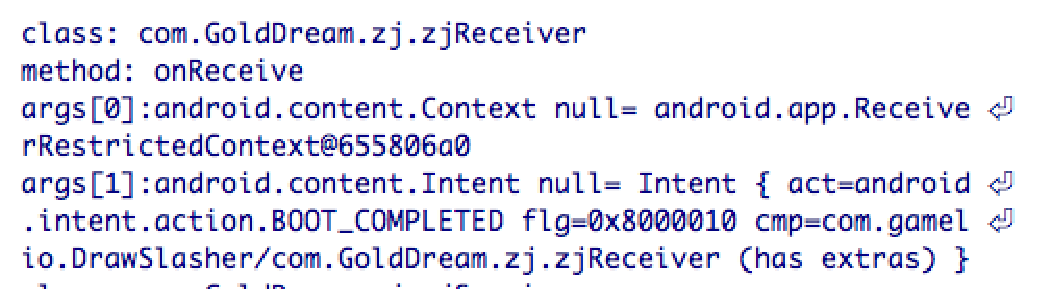
\includegraphics[scale=0.5]{onreceivezjservice.eps}
\end{center}
\caption{GoldDream の onReceive のログ}
\label{zjservicereceive}
\end{figure}

\begin{figure}[t]
\begin{center}
\graphicspath{{./epsfiles/}}
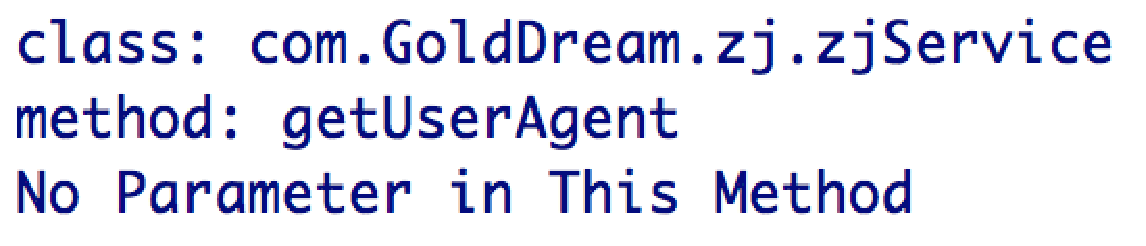
\includegraphics[scale=0.3]{getuseragentzjservice.eps}
\end{center}
\caption{GoldDream の getUserAgent のログ}
\label{zjserviceuseragent}
\end{figure}

\begin{figure}[t]
\begin{center}
\graphicspath{{./epsfiles/}}
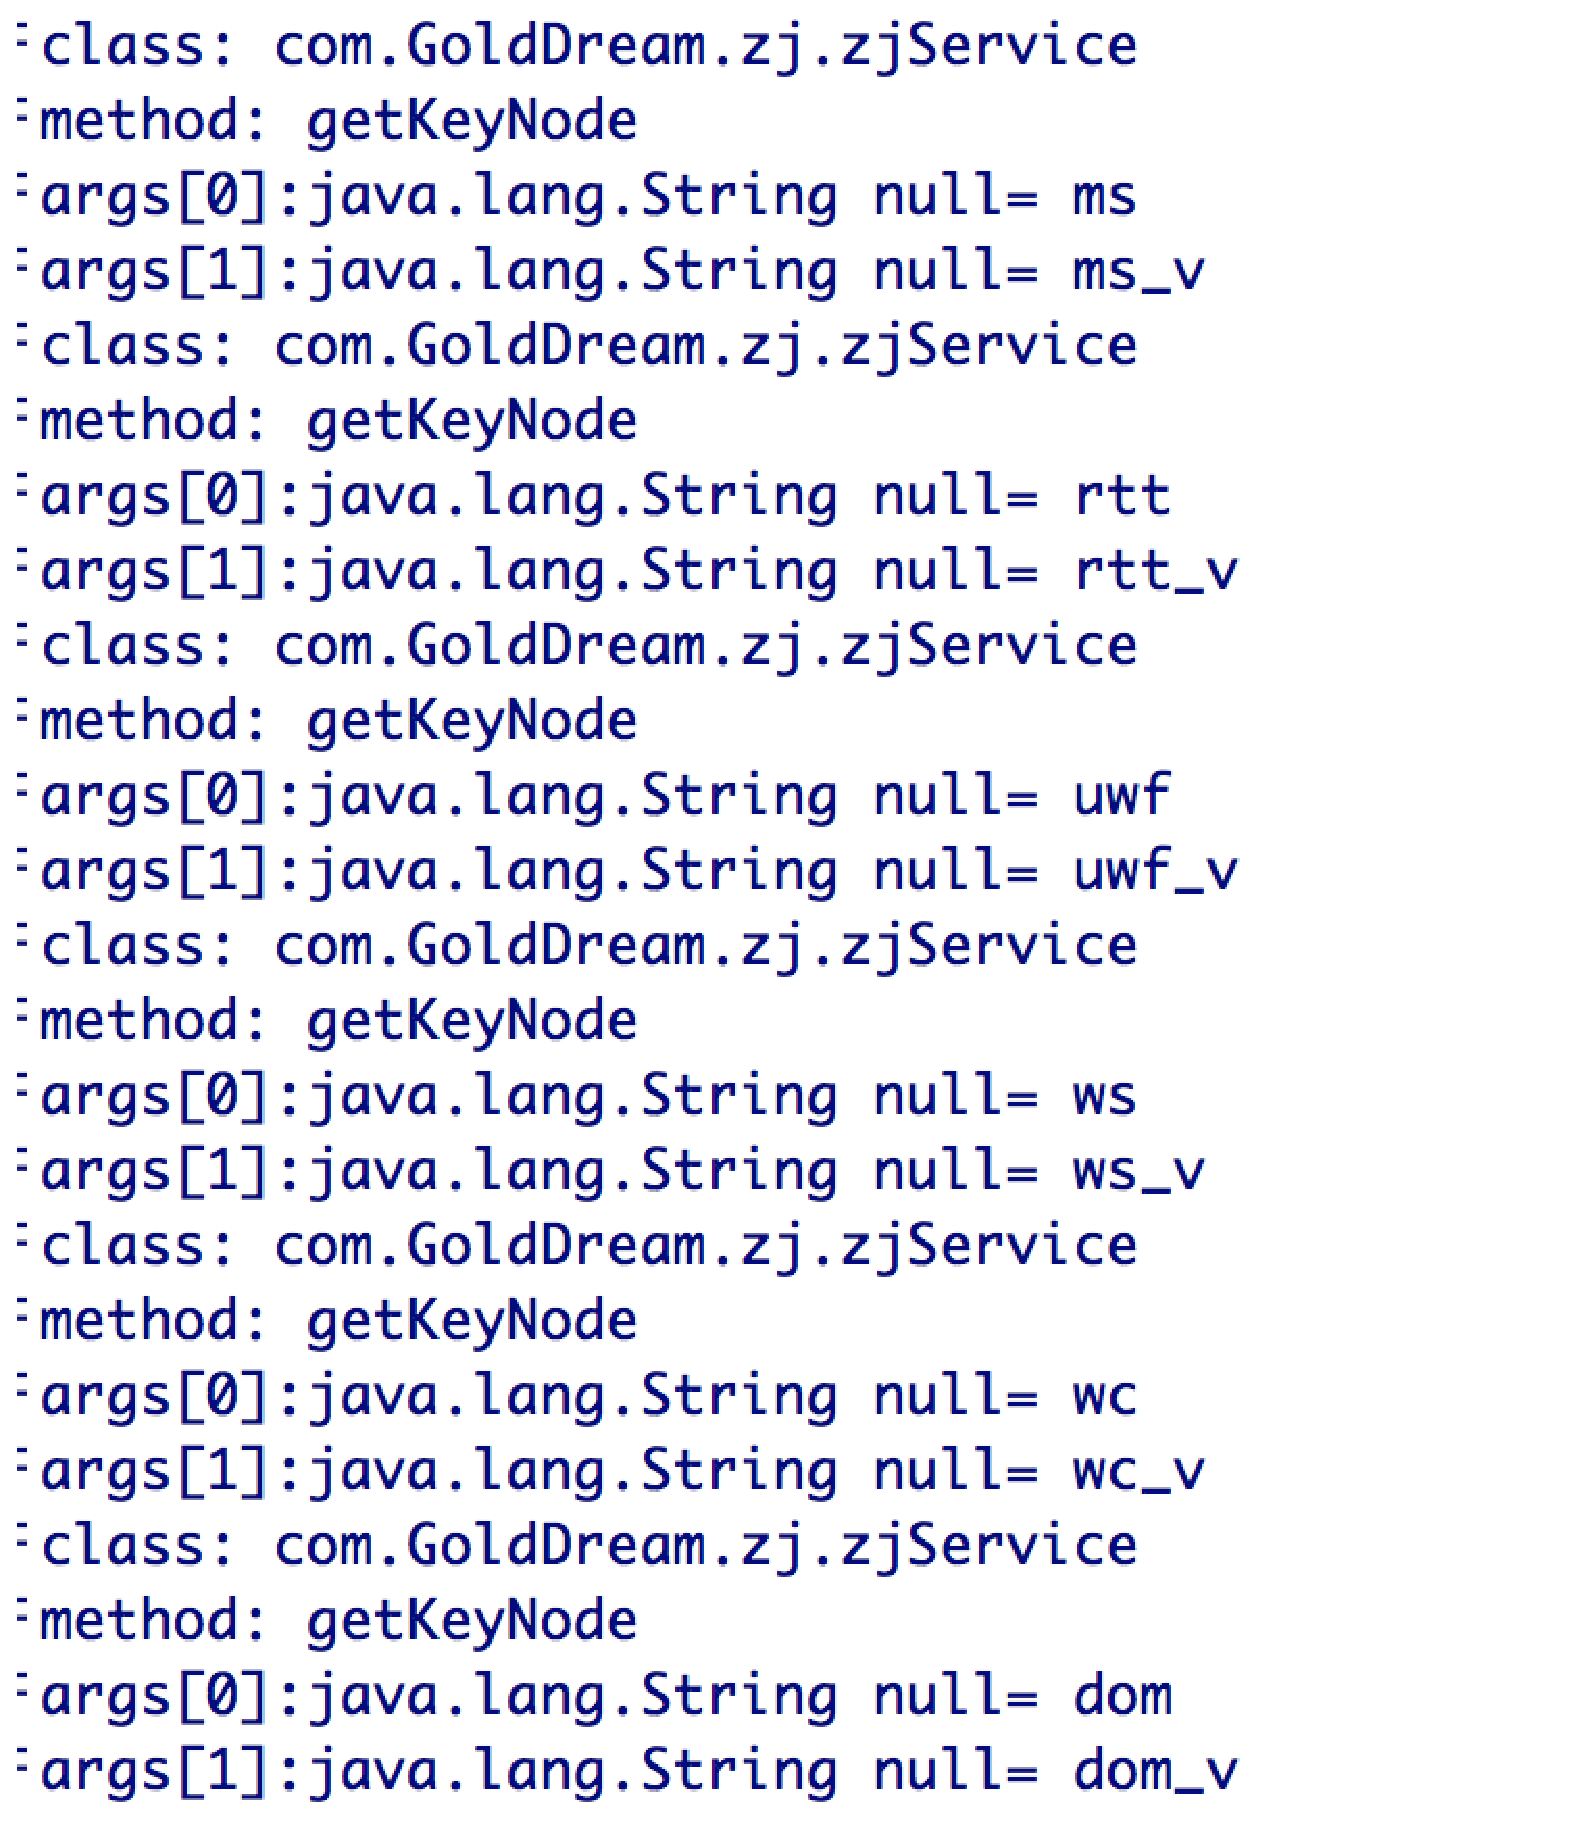
\includegraphics[scale=0.2]{getkeynodezjservice.eps}
\end{center}
\caption{GoldDream の getKeyNode のログ}
\label{zjservicegetkey}
\end{figure}

\begin{figure}[t]
\begin{center}
\graphicspath{{./epsfiles/}}
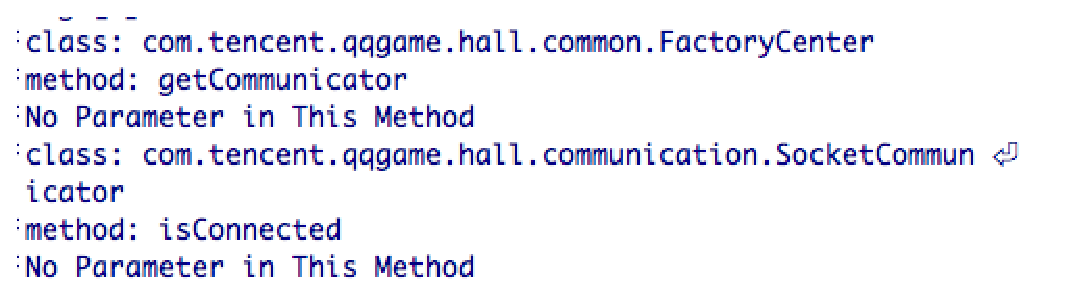
\includegraphics[scale=0.45]{qqgame.eps}
\end{center}
\caption{com.tencent.qqgame のメソッドのログ}
\label{qqgame}
\end{figure}

\begin{figure}[t]
\begin{center}
\graphicspath{{./epsfiles/}}
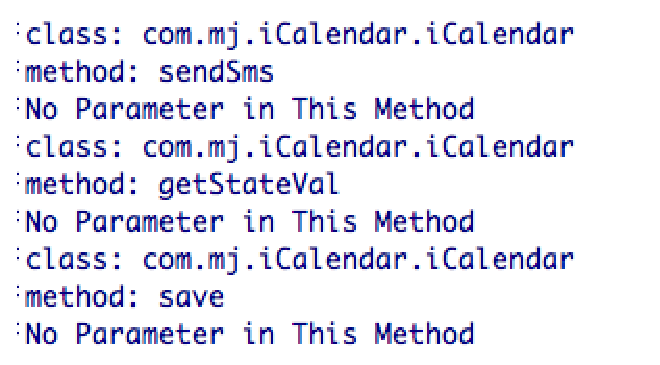
\includegraphics[scale=0.45]{icalendar1.eps}
\end{center}
\caption{iCalendar のメソッドのログ}
\label{calendar}
\end{figure}

\begin{figure}[t]
\begin{center}
\graphicspath{{./epsfiles/}}
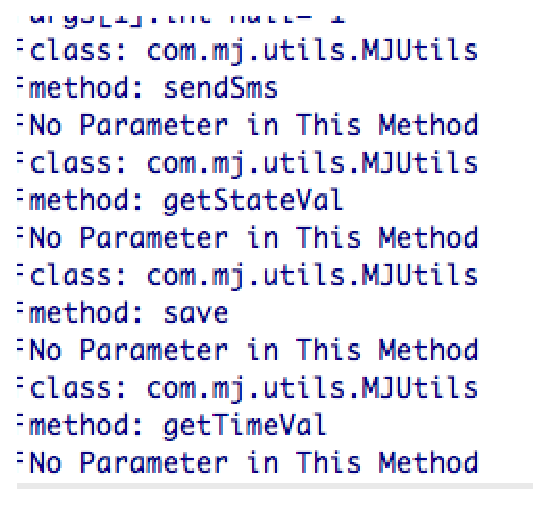
\includegraphics[scale=0.45]{imatch_sendsms.eps}
\end{center}
\caption{iMatch のメソッドのログ}
\label{imatch}
\end{figure}

\begin{figure}[t]
\begin{center}
\graphicspath{{./epsfiles/}}
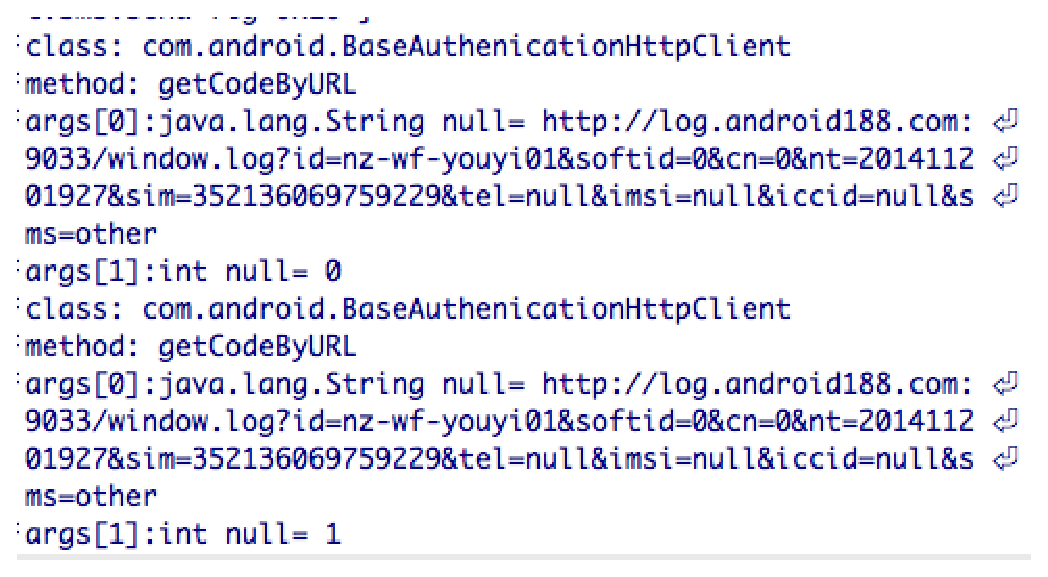
\includegraphics[scale=0.5]{baseauthentication_qq.eps}
\end{center}
\caption{com.tencent.qq の getCodeByURL のログ}
\label{qqauthentication}
\end{figure}


\begin{figure}[t]
\begin{center}
\graphicspath{{./epsfiles/}}
\includegraphics[scale=0.1]{nexus_qq_dialog.eps}
\end{center}
\caption{com.tencent.qq のダイアログ}
\label{dialog}
\end{figure}

\begin{figure}[t]
\begin{center}
\graphicspath{{./epsfiles/}}
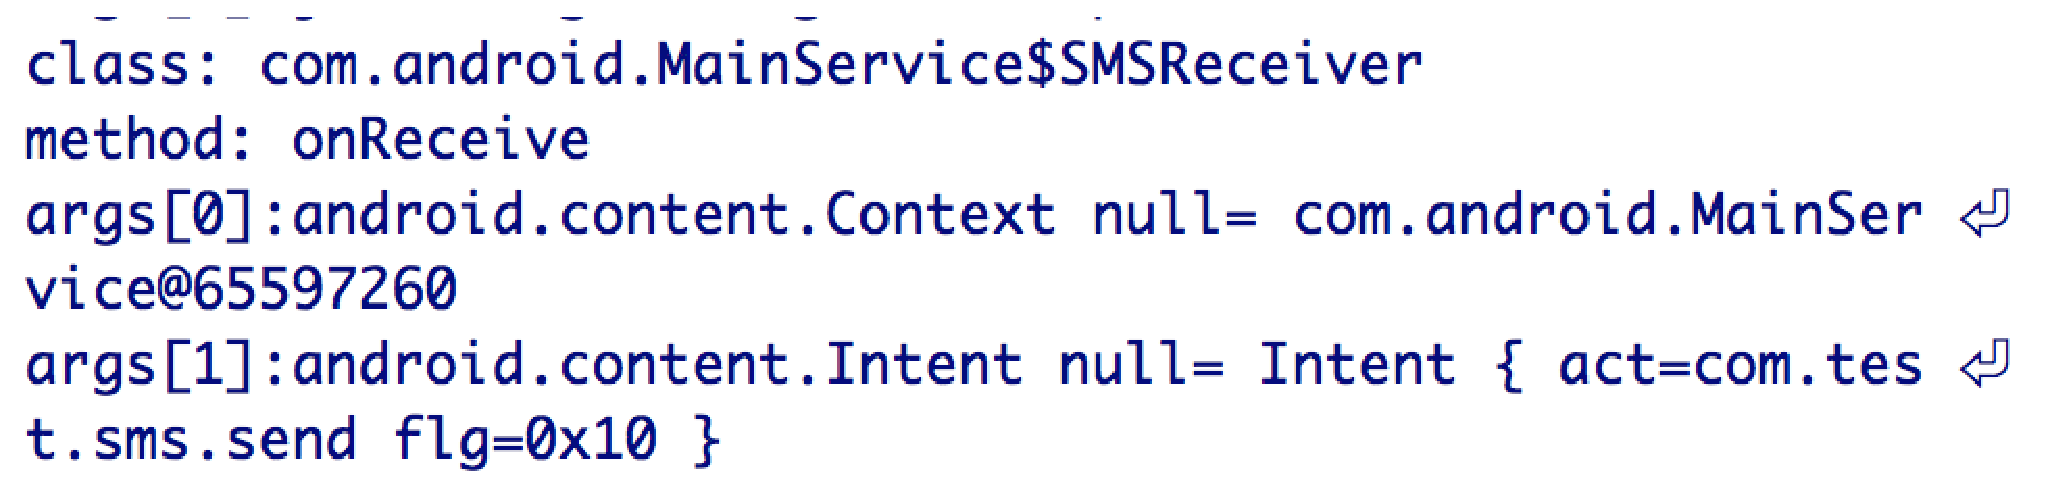
\includegraphics[scale=0.3]{SmsReceiver_qq.eps}
\end{center}
\caption{com.tencent.qqの onReceive のログ}
\label{qqreceive}
\end{figure}

Beauty Leg, Beauty Breast, Beauty Girl の 3 個のマルウェアからは,ログを得ることはできたが,図\ref{leg} のようにメソッド名が一文字のアルファベットであるためメソッドの内容を推測することができなかった,また,得られたメソッドのログの引数の中身を見ても,挙動を特定することができなかった.なお,図\ref{leg} の 1 つ目 (onCreate) と 3 つ目のメソッド (onStart) はそれぞれ android.app.Activity クラスのメソッドであり,全ての Android アプリは Activity クラスをオーバーライドしたクラスを持つ.そのため,onCreate, onStart はこのマルウェアの特有のメソッドではない.

不正な動きのログを得られなかったのは,これらのマルウェアのトリガーを再現できなかったためである.\ref{expmalware} で述べたように,この 3 つのマルウェアは電話の着信で起動する.モバイル端末は SIM カードがないと電話の発着信ができない.実験を行った Nexus 5 は SIM カードを挿入していなかったため,電話機能をもっていなかった.そのため,不正な振る舞いをするコードを実行することができなかった.


\begin{figure}[t]
\begin{center}
\graphicspath{{./epsfiles/}}
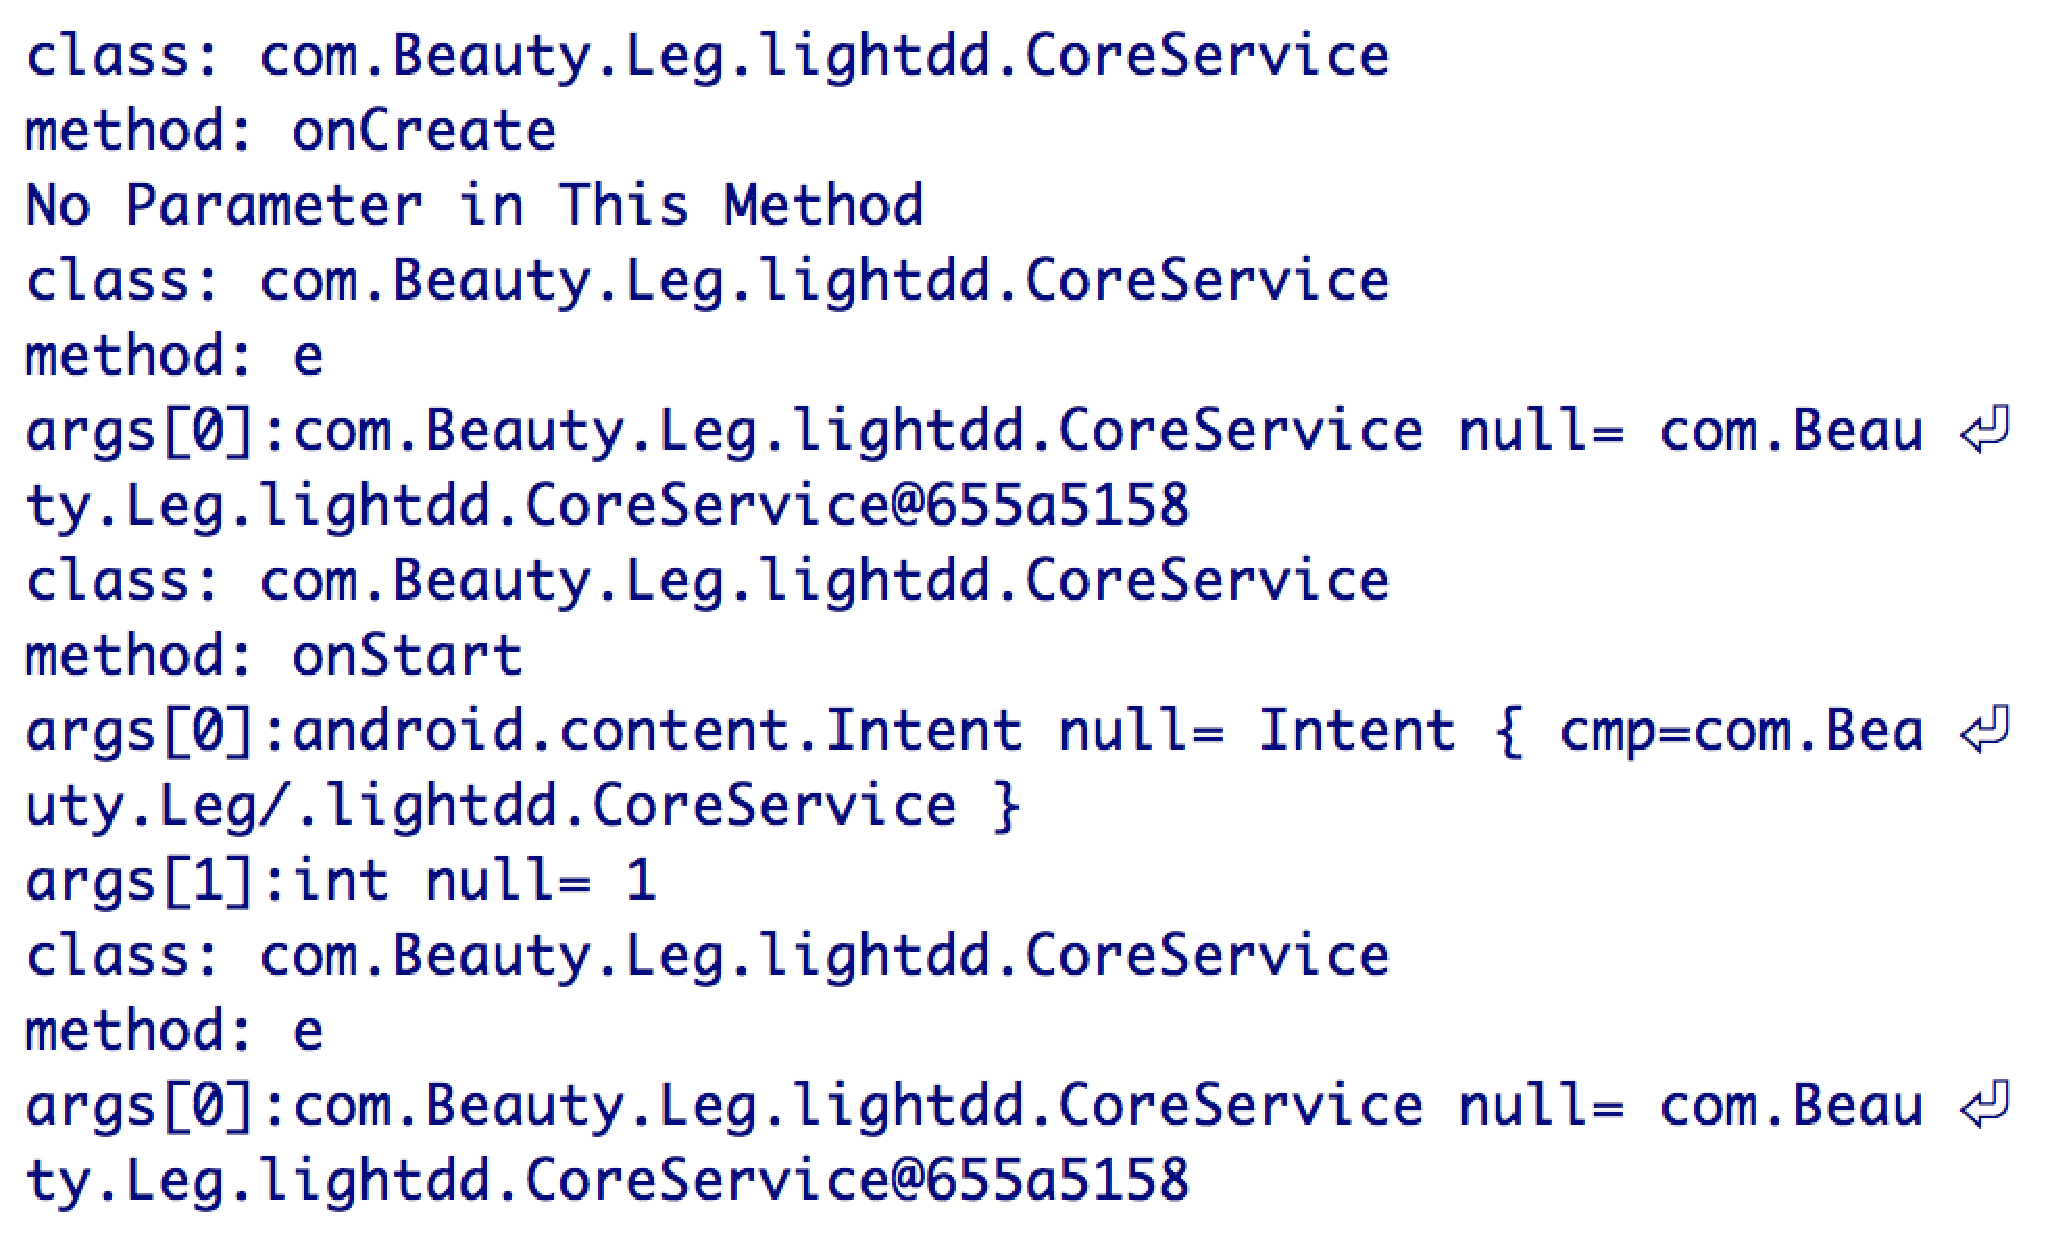
\includegraphics[scale=0.25]{beautyleg2.eps}
\end{center}
\caption{Beauty Leg のログ}
\label{leg}
\end{figure}

その他のマルウェアはログコードを挿入したにも関わらず,ログを得ることができなかった.その理由として,4 つ考えられる.ログコードを挿入した部分が少なかったことと,不正な動きそのものをしなかった,メソッド名を変えられた,一般的なメソッドで不正な動きをしている.

\subsubsection{実験 2 の結果}

